% (c) 2012 Claudio Carboncini - claudio.carboncini@gmail.com
% (c) 2012 Dimitrios Vrettos - d.vrettos@gmail.com
% (c) 2014 Daniele Zambelli - daniele.zambelli@gmail.com

\chapter{Calcolo letterale}

\section{Espressioni letterali e valori numerici}
\label{sec:esplett}

\subsection{Lettere per esprimere formule}

% \begin{exrig}
 \begin{esempio}
 In tutte le villette a schiera di recente costruzione del nuovo quartiere 
 Stella, vi è un terreno rettangolare di larghezza~\(12\unit{m}\) e 
 lunghezza~\(25\unit{m}\). Quanto misura la superficie del terreno?
\begin{center}
 % (c) 2012 Dimitrios Vrettos - d.vrettos@gmail.com
\begin{tikzpicture}[font=\small,x=10mm, y=5mm]

\draw[->] (0,0) -- (8,0) node [below right] () {$r$};
\node[above]  at (4,0) {3};
\begin{scope}[blue,thick]
\draw (0,0) -- (4,0);
\draw[fill=white] (4,0)circle (1.5pt);
\end{scope}

\end{tikzpicture}
\end{center}

Il prodotto delle dimensioni rappresenta la misura 
richiesta:~\(S=(25\cdot 12)m^{2}=300 m^2\).
 \end{esempio}
% \end{exrig}

Il semplice problema che abbiamo risolto è relativo ad un caso particolare; 
quel terreno con quelle dimensioni. Ma se le dimensioni fossero diverse?

La procedura per determinare la misura della superficie ovviamente è sempre 
la stessa e la possiamo esprimere con la formula~\(A=b\cdot h\) nella quale 
abbiamo indicato con~\(b\) la misura di una dimensione e con~\(h\) la misura 
dell'altra dimensione, assegnate rispetto alla stessa unità di misura.

\osservazione La formula ha carattere generale; essa serve ogni qualvolta 
si chiede di determinare la superficie di un rettangolo, note le misure 
delle dimensioni (base e altezza) rispetto alla stessa unità di misura.

In geometria si utilizzano tantissime formule che ci permettono di 
determinare perimetro e area delle figure piane, superficie laterale e 
totale 
e volume dei solidi. Nelle formule le lettere sostituiscono le misure di 
determinate grandezze, tipiche di quella figura o di quel solido.

% \ovalbox{\risolvi c}
\begin{comment}
\subsection{Lettere per descrivere schemi di calcolo}
% \begin{exrig}
 \begin{esempio}
 L'insegnante chiede agli alunni di scrivere 
 <<il doppio della somma di due numeri>>.

\begin{itemize*}
\item Antonella scrive:~\(2\cdot (3+78)\)
\item Maria chiede <<Quali sono i numeri? Se non li conosco non posso 
  soddisfare la richiesta>>;
\item Giulia scrive:~\(2\cdot (a+b)\).
\end{itemize*}
Maria si è posta il problema ma non ha saputo generalizzare la richiesta. 
Antonella si è limitata ad un caso particolare. 
Giulia ha espresso con una formula l'operazione richiesta dall'insegnante.
 \end{esempio}
% \end{exrig}

\osservazione L'uso di lettere dell'alfabeto per indicare numeri ci 
permette 
di generalizzare uno schema di calcolo.

\begin{definizione}
 Un'\emph{espressione letterale} o \emph{espressione algebrica} è uno 
schema 
 di calcolo in cui compaiono numeri e lettere legati dai simboli delle 
 operazioni.
\end{definizione}

Per scrivere un'espressione letterale ci si deve attenere a regole precise, 
quelle stesse che utilizziamo per scrivere espressioni numeriche.

Per esempio, la scrittura~``\(3\cdot 4+\)'' non è corretta, in quanto il 
simbolo~``\(+\)'' dell'addizione deve essere seguito da un altro numero per 
completare l'operazione. Analogamente non è corretta l'espressione 
letterale~``\(a\cdot c+\)''.

Come nelle espressioni numeriche, anche nelle espressioni letterali le 
parentesi indicano la priorità di alcune operazioni rispetto ad altre.
La formula~\(a\cdot (x+y)\) specifica ``il prodotto di un numero per la somma 
di 
due altri''. Essa è diversa da  \(a\cdot x+y\)
che rappresenta ``la somma del prodotto di due numeri con un terzo numero''.

% \vspazio\ovalbox{\risolvii \ref{ese:8.2}, \ref{ese:8.3}, \ref{ese:8.4}}

\subsection{Lettere per esprimere proprietà}

Le proprietà delle operazioni tra numeri si esprimono con lettere per 
indicare che valgono per numeri qualsiasi.
La scrittura~``\((a+b)+c=a+(b+c)\)'' per esempio esprime la proprietà 
associativa dell'addizione. In essa le lettere~\(a\), \(b\), \(c\) indicano
numeri qualsiasi. I due schemi di calcolo ci dicono che per sommare tre 
numeri è indifferente aggiungere alla somma dei primi due il terzo oppure 
aggiungere al primo la somma degli altri due.

% \vspazio\ovalbox{\risolvii \ref{ese:8.5}, \ref{ese:8.6}, \ref{ese:8.7}, 
% \ref{ese:8.8}, \ref{ese:8.9}, \ref{ese:8.10}, \ref{ese:8.11}, 
% \ref{ese:8.12}}

\end{comment}

\subsection{Valore numerico di un'espressione letterale}
\label{subsec:valnum}

Ogni espressione letterale rappresenta uno schema di calcolo in cui le 
lettere che vi compaiono sostituiscono numeri.
L'espressione letterale~\(2\cdot x^{2}+x\) traduce una catena di istruzioni 
che in linguaggio naturale sono così descritte: ``prendi un numero; 
fanne il quadrato; raddoppia quanto ottenuto; aggiungi al risultato 
il numero preso inizialmente''.

Questa catena di istruzioni si può anche rappresentare in modo schematico
\[x\rightarrow x^{2}\rightarrow~2\cdot x^{2}\rightarrow~2\cdot x^{2}+x\]
e può essere usata per istruire un esecutore a ``calcolare'' l'espressione 
letterale quando al posto della lettera~\(x\) si sostituisce un numero.

Calcoliamo il valore dell'espressione~\(2\cdot x^{2}+x\), sostituendo alla 
lettera il numero naturale~5.
Seguiamo la schematizzazione~\(x\rightarrow x^{2}\rightarrow~2\cdot 
x^{2}\rightarrow~2\cdot x^{2}+x\) e otteniamo:
\(5\rightarrow~25\rightarrow~50\rightarrow~55\).
Il risultato è~\(55\).
Più brevemente scriviamo~\(5\) nell'espressione letterale al posto di~\(x\): 
otteniamo l'espressione numerica~\(2\cdot 5^{2}+5\) il cui risultato è~\(55\).

E se al posto di~\(x\) sostituiamo~\(-5\)? Cambia il risultato?

Eseguiamo la sostituzione:  \(2\cdot (-5)^{2}+(-5)=\ldots\) Lasciamo a te il 
calcolo finale. Ti sarai accorto che il risultato è cambiato.

 \begin{definizione}
In un'espressione letterale le \emph{lettere} rappresentano 
le \emph{variabili} che assumono un preciso significato quando vengono 
sostituite da numeri.
Chiamiamo \emph{valore} di un'espressione letterale il risultato numerico 
che si ottiene eseguendo le operazioni indicate dallo
schema di calcolo quando alle lettere sostituiamo un numero. 
Il valore dell'espressione letterale dipende dal \emph{valore assegnato} 
alle sue variabili.
\end{definizione}

% \begin{exrig}
 \begin{esempio}
Calcolare il valore numerico dell'espressione:
\(3a(a-b)\) per~\(a = 1\), \(b = 1\).

\emph{Svolgimento}:~\(3\cdot 1\cdot (1-1)=3\cdot 1\cdot 0=0\).
\end{esempio}
 % \end{exrig}

% \ovalbox{\risolvii \ref{ese:8.13}, \ref{ese:8.14}, \ref{ese:8.15}, 
% \ref{ese:8.16}, \ref{ese:8.17}, \ref{ese:8.18}, \ref{ese:8.19}, 
% \ref{ese:8.20}, \ref{ese:8.21}, \ref{ese:8.22}, \ref{ese:8.23},
% \ref{ese:8.24}}

\begin{comment}

\subsection{Condizione di esistenza di un'espressione letterale}
\label{subsec:condes}

Ti proponiamo adesso alcuni casi particolari per
l'espressione~\(E=\dfrac{x-y}{3\cdot x}\).

\paragraph{Caso I}

\begin{center}
\begin{tabular*}{.2\textwidth}{@{\extracolsep{\fill}}*{3}{c}}
\toprule
\(x\) & \(y\) & \(E\)\\
1 & 1 & 0\\
\bottomrule
\end{tabular*}
\end{center}

Il numeratore della frazione è~0, mentre il denominatore vale~3; il
calcolo finale è dunque~\(\frac{0}{3}=0\).
Vi sono secondo te altre coppie che fanno
assumere ad~\(E\) quello stesso valore?

\paragraph{Caso II}
\begin{center}
\begin{tabular*}{.2\textwidth}{@{\extracolsep{\fill}}*{3}{c}}
\toprule
\(x\) &\(y\) &\(E\)\\
0 &25 &?\\
\bottomrule
\end{tabular*}
\end{center}

Invece di mettere un valore ad~\(E\), abbiamo messo punto di domanda
perché in questo caso il numeratore della frazione è~\(-25\) mentre
il denominatore vale~0; il calcolo finale è dunque~\(-{\frac{25}{0}}\), 
impossibile. Vi sono secondo te altre coppie che rendono
impossibile il calcolo del valore per~\(E\)?

Non possiamo allora concludere che per ogni coppia di numeri 
razionali~\((x,y)\) 
l'espressione~\(E\) assume un numero razionale.
Per poter calcolare il valore di~\(E\) non possiamo scegliere coppie 
aventi~\(x\) 
uguale a zero.
Scriveremo quindi come premessa alla ricerca dei valori di~\(E\) la 
\emph{Condizione di Esistenza}\,(\(\CE\))~\(x\neq~0\).

L'esempio appena svolto ci fa capire che di fronte a
un'espressione letterale dobbiamo riflettere sullo
schema di calcolo che essa rappresenta prima di assegnare valori alle
variabili che vi compaiono.

Se l'espressione letterale presenta una divisione in cui
il divisore contiene variabili, dobbiamo stabilire la~\(\CE\), 
eliminando quei valori che rendono nullo il divisore.
Per comprendere la necessità di porre le condizioni
d'esistenza ricordiamo la definizione di divisione.

Quanto fa~15 diviso~5? Perché? In forma matematica:~\(15:5=3\) perché \(3\cdot 
5=15\). Quindi, 
generalizzando~\(a:b=c\) se~\(c\cdot b=a\).

Vediamo ora cosa succede quando uno dei numeri è~0:

\begin{itemize*}
 \item quanto fa~0:5? Devo cercare un numero che moltiplicato per~5 mi 
dia~0: 
   trovo solo~0; infatti~\(0\cdot 5=0\).
 \item quanto fa~15:0? Devo cercare un numero che moltiplicato per~0 mi 
dia~15:
non lo trovo; infatti nessun numero moltiplicato per~0 fa~15. Quindi,
\(15:0\) è impossibile perché non esiste
\(x\) per il quale~\(x\cdot 0=15\).
 \item quanto fa~0:0? Devo cercare un numero che moltiplicato per~0 mi 
dia~0:
non ne trovo solo uno. Infatti, qualunque numero moltiplicato per~0
fa~0. Per esempio, \(0:0=33\) infatti
\(33\cdot 0=0\). Anche~\(0:0=-189,6\)
infatti~\(-189,6\cdot 0=0\). Anche \(0:0=0\)
infatti~\(0\cdot 0=0\). 
Ancora~\(0:0=10^{99}\) infatti~\(10^{99}\cdot 0=0\).
Quindi~\(0:0\) è indeterminato, perché
non è possibile determinare un~\(x\) tale che~\(x\cdot 0=0\),
per qualunque valore di~\(x\) si ha~\(x\cdot 0=0\).
\end{itemize*}

Consideriamo l'espressione letterale~\(E=\frac{a-b}{a+b}\) dove~\(a\) e~\(b\) 
rappresentano numeri razionali.
Premettiamo:

\begin{enumeratea}
 \item la descrizione a parole dello schema di calcolo:
``divisione tra la differenza di due numeri e la loro
somma'';
 \item la domanda che riguarda il denominatore: ``quando
sommando due numeri razionali otteniamo~0 al
denominatore?'';
 \item la~\(\CE\): ``\(a\) e~\(b\) non devono essere numeri opposti''.
\end{enumeratea}

Siamo ora in grado di completare la tabella:
\begin{center}
\begin{tabular*}{.8\textwidth}{l@{\extracolsep{\fill}}*{5}{c}}
\toprule
\(a\) & 3 &0 & \(\frac{3}{4}\) &\(-{\frac{5}{8}}\) & \(-{\frac{19}{2}}\) \\
\(b\) & \(-3\) & \(-{\frac{1}{2}}\) & 0 &\(\frac{5}{8}\) & \(-{\frac{19}{2}}\) 
\\
\midrule
\(E=\frac{a-b}{a+b}\) & & & & &\\
\bottomrule
\end{tabular*}
\end{center}

Dalla~\(\CE\), ci accorgiamo subito che la
prima coppia e la quarta sono formate da numeri opposti, pertanto non
possiamo con esse calcolare il valore di~\(E\). L'ultima
coppia è formata da numeri uguali pertanto la loro differenza è~0;
il numeratore si annulla e quindi il valore di~\(E\) è~0. 
Per la coppia~\(\tonda{0,-\frac{1}{2}}\) il valore di~\(E\) è~\(-1\) 
mentre 
è~1 per la coppia~\(\tonda{\frac{3}{4},0}\).
La tabella verrà quindi così completata:

\begin{center}
\begin{tabular*}{.8\textwidth}{l@{\extracolsep{\fill}}*{5}{c}}
\toprule
\(a\) & 3 &0 & \(\frac{3}{4}\) &\(-{\frac{5}{8}}\) & \(-{\frac{19}{2}}\) \\
\(b\) & \(-3\) & \(-{\frac{1}{2}}\) & 0 &\(\frac{5}{8}\) & \(-{\frac{19}{2}}\) 
\\
\midrule
\(E\) &impossibile & \(-1\)& 1& impossibile&0\\
\bottomrule
\end{tabular*}
\end{center}

Cosa succede per la coppia~(0,0)?

% \vspazio\ovalbox{\risolvii \ref{ese:8.25}, \ref{ese:8.26}, 
% \ref{ese:8.27}, \ref{ese:8.28}, \ref{ese:8.29}, \ref{ese:8.30}, 
% \ref{ese:8.31}, \ref{ese:8.32}}
\end{comment}

% (c) 2012-2014 Dimitrios Vrettos - d.vrettos@gmail.com
% (c) 2014 Daniele Zambelli - daniele.zambelli@gmail.com

\section{I monomi}
\label{sec:09_monomi}

\subsection{Definizioni}
\label{subsec:09_monomi_definizioni}

D'ora in poi quando scriveremo un'espressione letterale in cui compare
l'operazione di moltiplicazione, tralasceremo il puntino fin qui usato per 
evidenziare l'operazione.
Così l'espressione~\(5\cdot a^{2}+\frac{3}{8}\cdot a\cdot b-7\cdot b^{2}\) 
verrà scritta in modo
più compatto~\(5a^{2}+\frac{3}{8}ab-7b^{2}\).

% \begin{definizione}
% Una espressione letterale in cui numeri e lettere sono legati dalla sola 
% moltiplicazione si chiama \emph{monomio}.
% \end{definizione}
% 
% % \begin{exrig}
%  \begin{esempio}
% L'espressione nelle due variabili~\(a\) e~\(b\), \(E=5\cdot 
% 2a^{2}\frac{3}{8}ab7b^{2}\)
% è un monomio perché numeri e lettere sono legate solo dalla moltiplicazione.
%  \end{esempio}

\begin{definizione}
Chiamiamo \emph{monomio} una espressione letterale in cui non compare 
l'addizione algebrica.
\end{definizione}

% \begin{exrig}
 \begin{esempio}
L'espressione nelle due variabili~\(a\) e~\(b\), \(E=5\cdot 
2a^{2}\frac{3}{8}ab7b^{2}\)
è un monomio perché nell'espressione non appaiono addizioni o sottrazioni.
 \end{esempio}

 \begin{esempio}
L'espressione~\(E=2a^{2}-ab^{2}\) non è un monomio poiché compare anche il 
segno di sottrazione.
 \end{esempio}
% \end{exrig}

% \ovalbox{\risolvi \ref{ese:9.1}}

\osservazione
Gli elementi di un monomio sono \emph{fattori}, perché sono termini
di una moltiplicazione ma possono comparire anche \emph{potenze},
infatti la potenza è una moltiplicazione di fattori uguali. 
% Non possono invece comparire esponenti negativi o frazionari. 
% In un monomio gli esponenti delle variabili devono essere numeri naturali.

\begin{definizione}
Un monomio si dice \emph{ridotto in forma normale} quando è scritto come 
prodotto di un solo fattore numerico e di potenze letterali con basi 
diverse.
\end{definizione}

% \begin{exrig}
 \begin{esempio}
Il monomio~\(E=5\cdot a^{2}\frac{3}{20}ab6b^{2}\) non è scritto in
forma normale: tra i suoi fattori vi sono numeri diversi e le potenze
letterali hanno basi ripetute, la~\(a\) e la~\(b\) compaiono due volte ciascuna.

Moltiplichiamo tra loro i fattori numerici e otteniamo~\(\frac{9}{2}\) 
eseguiamo il prodotto di potenze con la stessa base otteniamo
\(a^{3}b^{3}\). Il monomio in forma normale è~\(E=\frac{9}{2}a^{3}b^{3}\).
 \end{esempio}
% \end{exrig}

\begin{procedura}
 Ridurre in forma normale un monomio:
 \begin{enumeratea}
 \item moltiplicare tra loro i fattori numerici;
 \item moltiplicare le potenze con la stessa base.
 \end{enumeratea}
\end{procedura}

% \ovalbox{\risolvi \ref{ese:9.2}}

\begin{definizione}
Chiamiamo \emph{coefficiente} la parte numerica del monomio ridotto a forma 
normale.
\end{definizione}

\begin{definizione}
Chiamiamo \emph{parte letterale} il complesso delle lettere che compaiono 
nel monomio ridotto a forma normale.
\end{definizione}

% \begin{exrig}
 \begin{esempio}
 Nella tabella seguente sono segnati alcuni monomi e i rispettivi 
coefficienti.
\begin{center}
 \begin{tabular}{lcccc}
 \toprule
 monomio & \(-{\frac{1}{2}}abc\) & \(3x^{3}y^{5}\) & \(a^{5}b^{7}\) & 
\(-k^{2}\)\\
coefficiente & \(-{\frac{1}{2}}\) & \(3\) & \(1\) & \(-1\) \\
parte letterale & \(abc\) & \(x^{3}y^{5}\) & \(a^{5}b^{7}\) & \(k^{2}\) \\
 \bottomrule
\end{tabular}
\end{center}
 \end{esempio}
% \end{exrig}

Se il coefficiente del monomio è zero il \emph{monomio} si dice 
\emph{nullo}.

Se in un monomio non appare il coefficiente è sottinteso che il 
coefficiente sia~1: \(a^5b = 1 a^5b\)

% % \begin{exrig}
%  \begin{esempio}
% L'espressione letterale~\(\frac{3}{5}a^{3}bc^{2}\) è un monomio;
% il numero~\(\frac{3}{5}\) e le lettere~\(a^{3}\), \(b\), \(c^{2}\) sono legate
% dall'operazione di moltiplicazione; il suo coefficiente è il 
% numero~\(\frac{3}{5}\) e la parte letterale è~\(a^{3}bc^{2}\).
%  \end{esempio}
% 
%  \begin{esempio}
%  Controesempi:
% 
%  \begin{enumeratea}
%  \item l'espressione letterale~\(\frac{3}{5}a^{3}+bc^{2}\)
%  non è un monomio dal momento che numeri e lettere sono legati oltre
% che dalla moltiplicazione anche dalla addizione;
% \item l'espressione letterale~\(\frac{3}{5}a^{-3}bc^{2}\)
% non è un monomio in quanto la potenza con esponente negativo
% rappresenta una divisione, infatti~\(a^{-3}=\frac{1}{a^{3}}\).
% \end{enumeratea}
%  \end{esempio}
% % \end{exrig}

\begin{definizione}
Diciamo che un monomio è \emph{intero} se non ha lettere al denominatore 
(o, che è equivalente, se le lettere non hanno esponenti negativi) 
altrimenti si dice \emph{fratto}.
\end{definizione}

% \begin{exrig}
 \begin{esempio}
Il monomio~\(\dfrac{3}{5}a^{3}bc^{2}\) è intero,\\ 
il monomio~\(\dfrac{3}{5}a^{-3}b^{-1}c^{2}=
             \dfrac{3}{5}\dfrac{c^{2}}{a^{3}b} =
             \dfrac{3c^{2}}{5a^{3}b}\) è fratto.
 \end{esempio}
% \end{exrig}

\begin{definizione}
Diciamo che due o più monomi sono \emph{simili} se hanno parte letterale 
identica.
\end{definizione}

% \begin{exrig}
 \begin{esempio}
Il monomio~\(\frac{3}{5}a^{3}bc^{2}\) è simile
a~\(68a^{3}bc^{2}\) e anche a~\(-0,5a^{3}bc^{2}\), ma non è simile
a~\(\frac{3}{5}a^{2}bc^{3}\). L'ultimo monomio ha le
stesse lettere degli altri ma sono elevate ad esponenti diversi.
 \end{esempio}
% \end{exrig}

\osservazione Il monomio nullo si considera simile a qualunque altro 
monomio.

\begin{definizione}
Si dicono \emph{opposti} due monomi simili che hanno coefficiente opposto.
\end{definizione}

% \begin{exrig}
 \begin{esempio}
I monomi~\(\frac{3}{5}a^{3}bc^{2}\) e~\(-{\frac{3}{5}}a^{3}bc^{2}\) sono 
opposti, infatti sono simili e hanno coefficienti opposti.
\end{esempio}

\begin{esempio}
Non sono opposti~\(\frac{3}{5}a^{3}bc^{2}\) e~\(-7a^{3}bc^{2}\) ma 
semplicemente simili. I loro coefficienti hanno segno diverso, ma
non sono numeri opposti.
\end{esempio}
% \end{exrig}

% \ovalbox{\risolvi \ref{ese:9.3}}

\begin{definizione}
Il \emph{grado complessivo} di un monomio è la somma degli esponenti della 
parte letterale.

Quando il monomio è ridotto a forma normale, l'esponente di una sua 
variabile ci indica il
\emph{grado} del monomio \emph{rispetto a quella variabile}.
\end{definizione}

% \begin{exrig}
 \begin{esempio}
Il monomio~\(\frac{3}{5}a^{3}bc^{2}\) ha grado complessivo~6,
ottenuto sommando gli esponenti della sua parte letterale~\((3+1+2=6)\).
Rispetto alla variabile~\(a\) è di terzo grado, rispetto alla
variabile~\(b\) è di primo grado, rispetto alla variabile
\(c\) è di secondo grado.
 \end{esempio}
% \end{exrig}

% Abbiamo detto che gli esponenti della parte letterale del monomio sono
% numeri naturali, dunque possiamo anche avere una o più variabili
% elevate ad esponente~0. Cosa succede allora nel monomio?
% 
% Consideriamo il monomio~\(56a^{3}b^{0}c^{2}\), sappiamo che qualunque
% numero diverso da zero elevato a zero è uguale a~1, quindi possiamo
% sostituire la variabile~\(b\) che ha esponente~0 con~1 e
% otteniamo~\(56a^{3}\cdot 1\cdot c^{2}=56a^{3}c^{2}\). Se in un monomio ogni
% variabile ha esponente~0, il monomio rimane solamente con il suo
% coefficiente numerico: per esempio~\(-3a^{0}x^{0}=-3\cdot 1\cdot 1=-3\).

\osservazione Esistono \emph{monomi di grado~0}; essi presentano solo il
coefficiente e pertanto \emph{sono} equiparabili ai \emph{numeri razionali}.

\subsection{Valore di un monomio}
\label{subsec:09_monomi_valore}

Poiché il monomio è un'espressione letterale,
possiamo calcolarne il valore quando alle sue variabili sostituiamo numeri.

% \begin{exrig}
 \begin{esempio}
 Calcola il valore del monomio~\(3x^{4}y^{5}z\) per i valori~\(x=-3\), \(y=5\) 
e~\(z=0\).

Sostituendo i valori assegnati otteniamo~\(3\cdot (-3)^{4}\cdot 5^{5}\cdot 
0=0\) essendo uno dei fattori nullo.
 \end{esempio}
% \end{exrig}

\osservazione Il valore di un monomio è nullo quando almeno una delle sue 
variabili assume il valore~0.

Molte formule di geometria sono scritte sotto forma di monomi: area del
triangolo~\(\frac{1}{2}bh\) area del quadrato~\(l^{2}\)
perimetro del quadrato~\(4l\) area del rettangolo~\(bh\) volume del 
cubo~\(l^{3}\) ecc.
Esse acquistano significato quando alle lettere sostituiamo
numeri che rappresentano le misure della figura considerata.

% \ovalbox{\risolvii \ref{ese:9.4}, \ref{ese:9.5}, \ref{ese:9.6}, 
% \ref{ese:9.7}, \ref{ese:9.8}, \ref{ese:9.9}, \ref{ese:9.10}, 
% \ref{ese:9.11}, \ref{ese:9.12}}

\subsection{Moltiplicazione di monomi}
\label{subsec:09_monomi_prodotto}

Ci proponiamo ora di introdurre nell'insieme dei monomi
le operazioni di addizione, sottrazione, moltiplicazione, potenza,
divisione.

Ricordiamo che definire in un insieme un'operazione
significa stabilire una legge che associa a due elementi
dell'insieme un altro elemento
dell'insieme stesso.

La moltiplicazione di due monomi si indica con lo stesso simbolo della
moltiplicazione tra numeri; i suoi termini si chiamano fattori e il
risultato si chiama prodotto, proprio come negli insiemi numerici.
Dato che nella moltiplicazione vale la proprietà commutativa:

\begin{definizione}
 Il prodotto di due monomi è il monomio avente
per coefficiente il prodotto dei coefficienti e per parte letterale il
prodotto delle parti letterali.
\end{definizione}

% \begin{exrig}
 \begin{esempio}
Assegnati i monomi~\(m_{1}=-4x^{2}yz^{3}\) e~\(m_{2}=\frac{5}{6}x^{3}z^{6}\)
il monomio prodotto è
\[m_{1} \cdot m_{2}=\tonda{-4x^{2}yz^{3}} \tonda{\frac{5}{6}x^{3}z^{6}}=
\bigg(-4\cdot {\frac{5}{6}}\bigg)\tonda{x^{2}\cdot x^{3}}\cdot 
y\cdot \tonda{z^{3}\cdot z^{6}}=-\frac{10}{3}x^{5}yz^{9}.\]
 \end{esempio}
% \end{exrig}


% \begin{procedura}[per moltiplicare due monomi]
% La moltiplicazione tra monomi si effettua moltiplicando prima i
% coefficienti numerici e dopo le parti letterali:
% 
% \begin{enumeratea}
%  \item nella moltiplicazione tra i coefficienti usiamo le regole note della
% moltiplicazione tra numeri razionali;
%  \item nella moltiplicazione tra le parti letterali applichiamo la regola
% del prodotto di potenze con la stessa base.
% \end{enumeratea}
% \end{procedura}

% \subsubsection{Proprietà della moltiplicazione}
% 
% \begin{enumeratea}
% \item commutativa:~\(m_{1}\cdot m_{2}=m_{2}\cdot m_{1}\)
% \item associativa:~\(m_{1}\cdot m_{2}\cdot m_{3}=(m_{1}\cdot m_{2})\cdot 
% m_{3}=m_{1}\cdot (m_{2}\cdot m_{3})\)
% \item 1 è l'elemento neutro:~\(1\cdot m=m\cdot 1=m\)
% \item se uno dei fattori è uguale a~0 il prodotto è~0, cioè~\(0\cdot 
% m=m\cdot 0=0\).
% \end{enumeratea}

% \ovalbox{\risolvii \ref{ese:9.13}, \ref{ese:9.14}, \ref{ese:9.15}, 
% \ref{ese:9.16}}

\subsection{Potenza di un monomio}
\label{subsec:09_monomi_potenza}

% Ricordiamo che tra i numeri l'operazione di elevamento a
% potenza ha un solo termine, la base, sulla quale si agisce a seconda
% dell'esponente.
% 
% \[\text{Potenza }=\text{ base }^\text{ esponente}= \underbrace{(\text{ base 
% }\cdot \text{ base }\cdot\text{ base }\cdot\ldots\cdot \text{ base 
% })}_{\text{tanti fattori quanti ne indica l'esponente}}.\]
% 
% Analogamente viene indicata la potenza di un monomio: la base è un
% monomio e l'esponente è un numero naturale.

\begin{definizione}
La \emph{potenza di un monomio} è un monomio
che ha per coefficiente la potenza del coefficiente e per parte
letterale la potenza della parte letterale.
\end{definizione}

% \begin{exrig}
 \begin{esempio}
Calcoliamo il quadrato e il cubo del monomio~\(m_{1}=-{\frac{1}{2}}a^{2}b\).
\begin{align*}
\bigg(-{\frac{1}{2}}a^{2}b\bigg)^{2}
&=\bigg(-{\frac{1}{2}}\bigg)^{2}\cdot\tonda{a^{2}}^{2}\cdot (b)^{2}
=\frac{1}{4}a^{4}b^{2}
\end{align*}
\begin{align*}
\bigg(-{\frac{1}{2}}a^{2}b\bigg)^{3}
&=\bigg(-{\frac{1}{2}}\bigg)^{3}\cdot\tonda{a^{2}}^{3}\cdot (b)^{3}
=-{\frac{1}{8}}a^{6}b^{3}
\end{align*}
 \end{esempio}

 \begin{esempio}
Calcoliamo il quadrato e il cubo del monomio~\(m_{2}=5a^{3}b^{2}c^{2}\).
\begin{align*}
\tonda{5a^{3}b^{2}c^{2}}^{2}
&=\tonda{5}^{2}\cdot \tonda{a^{3}}^{2}\cdot\tonda{b^{2}}^{2}\cdot 
\tonda{c^{2}}^{2}
=25a^{6}b^{4}c^{4}
\end{align*}
\begin{align*}
\tonda{5a^{3}b^{2}c^{2}}^{3}
&=\tonda{5}^{3}\cdot \tonda{a^{3}}^{3}\cdot\tonda{b^{2}}^{3}\cdot 
\tonda{c^{2}}^{3}
=125a^{9}b^{6}c^{6}
\end{align*}
 \end{esempio}
% \end{exrig}

% \begin{procedura}
% Eseguire la potenza di un monomio:
% 
% \begin{enumeratea}
%  \item applichiamo la proprietà relativa alla potenza di un prodotto,
% eseguiamo cioè la potenza di ogni singolo fattore del monomio;
%  \item applichiamo la proprietà relativa alla potenza di potenza,
% moltiplicando l'esponente della variabile per l'esponente delle potenza.
% \end{enumeratea}
% \end{procedura}

% \ovalbox{\risolvii \ref{ese:9.17}, \ref{ese:9.18}, \ref{ese:9.19}, 
% \ref{ese:9.20}}

\subsection{Divisione di due monomi}
\label{subsec:09_monomi_quoziente}

Premessa: ricordiamo che il quoziente della divisione tra un dividendo \(n\) 
e un divisore \(d\) è il numero \(q\) che moltiplicato per il divisore dà come 
risultato il dividendo:
\[n : d = q \sLRarrow q \cdot d = n\]

Con i numeri razionali la divisione si trasforma nella moltiplicazione tra 
il dividendo e il reciproco del divisore:
\[n : d = n \cdot \frac{1}{d}\]

Possiamo usare la stessa regola anche per i monomi se prima definiamo cosa 
è il reciproco di un monomio:

\begin{definizione}
Il \emph{reciproco} di un monomio è il monomio che si ottiene moltiplicando 
il reciproco del coefficiente con il reciproco della parte letterale.
\end{definizione}

\begin{esempio}
 il reciproco di \(\dfrac{3}{4}a^3bc^2\) \quad è\\
\(\dfrac{4}{3}\dfrac{1}{a^3bc^2}\) \quad o anche \quad
\(\dfrac{4}{3a^3bc^2}\) \quad o anche \quad
\(\dfrac{4}{3}a^{-3}b^{-1}c^{-2}\)
\end{esempio}

\begin{definizione}
Il \emph{quoziente} tra due monomi si ottiene moltiplicando il primo per il 
reciproco del secondo.
\end{definizione}

% \begin{exrig}
 \begin{esempio}
Calcola: \(\tonda{36x^{5}y^{2}}:\tonda{-18x^{3}y}\)
\[\tonda{36x^{5}y^{2}}:\tonda{-18x^{3}y} =
\tonda{36x^{5}y^{2}} \cdot \tonda{\frac{-1}{18x^{3}y}} =-2x^{2}y\]
Infatti~\((-2x^{2}y)\cdot(-18x^{3}y)=(36x^{5}y^{2})\).
 \end{esempio}
% % \end{exrig}
% 
% \begin{procedura}[Calcolare il quoziente di due monomi]
% Il quoziente di due monomi è così composto:
% 
% \begin{enumeratea}
%  \item il coefficiente è il quoziente dei coefficienti dei monomi dati;
%  \item la parte letterale ha gli esponenti ottenuti sottraendo gli esponenti
% delle stesse variabili;
%  \item se la potenza di alcune lettere risulta negativa il risultato della
% divisione non è un monomio.
% \end{enumeratea}
% \end{procedura}
% 
% % \begin{exrig}
 \begin{esempio}
\(\tonda{\frac{7}{2}a^{3}x^{4}y^{2}}:\tonda{-\frac{21}{8}ax^{2}y}\).
\[\tonda{\frac{7}{2}a^{3}x^{4}y^{2}}:\tonda{-\frac{21}{8}ax^{2}y} =
  \tonda{\frac{7}{2}a^{3}x^{4}y^{2}}\cdot \tonda{-\frac{8}{21ax^{2}y}} =
-\frac{4}{2}a^{2}x^{2}y\]
Dato che la divisione è definita solo se il divisore è diverso da 0, il 
risultato ottenuto è valido solo se:
\(a \neq 0 \text{ e } x \neq 0 \text{ e } y\neq 0\)
 \end{esempio}

 \begin{esempio}
\(\tonda{\frac{9}{20}a^{2}b^{4}}:\tonda{-{\frac{1}{8}}a^{5}b^{2}}\)

Si può eseguire la divisione solo se~\(a\neq~0\text{ e }b\neq~0\), 
In questo caso:
\[\tonda{\frac{9}{20}a^{2}b^{4}}:\tonda{-{\frac{1}{8}}a^{5}b^{2}} =
\tonda{\frac{9}{20}a^{2}b^{4}} \cdot \tonda{-\frac{8}{a^{5}b^{2}} =
-\frac{18b^2}{5a^3} = -\frac{18}{5}}\frac{b^2}{a^3}\]
con: 
\(a \neq 0 \text{ e } b \neq 0\)
 \end{esempio}
% \end{exrig}

% In conclusione, l'operazione di divisione tra due monomi
% ha come risultato un monomio se ogni variabile del dividendo ha
% esponente maggiore o uguale all'esponente con cui
% compare nel divisore.


% \vspazio\ovalbox{\risolvii \ref{ese:9.21}, \ref{ese:9.22}, \ref{ese:9.23}}

\subsection{Addizione di due monomi}
\label{subsec:09_monomi_somma}

Di solito quando si affrontano le operazioni, si parte dall'addizione, 
invece con i monomi l'abbiamo tenuta per ultima perché non sempre la somma 
di due monomi è un monomio: l'addizione di monomi non è una legge di 
composizione interna.

\begin{definizione}
La \emph{somma algebrica di due monomi simili} è un monomio simile agli 
addendi che ha come coefficiente la somma algebrica dei coefficienti.
\end{definizione}

% \begin{exrig}
 \begin{esempio}
Calcoliamo~\(3x^{3}+(-6x^{3})\).

I due addendi sono monomi simili dunque la somma è ancora un monomio
ed è simile ai singoli addendi. Precisamente
\(3x^{3}+(-6x^{3})=(3+(-6))x^{3}=-3x^{3}\).

Osserva che la somma di monomi simili si riduce alla somma algebrica di 
numeri.
 \end{esempio}
% \end{exrig}

% \ovalbox{\risolvi \ref{ese:9.24}}

% \subsubsection{Proprietà della addizione}
% 
% \begin{enumeratea}
%  \item commutativa:~\(m_{1}+m_{2}=m_{2}+m_{1}\)
%  \item 
% associativa:~\(m_{1}+m_{2}+m_{3}=(m_{1}+m_{2})+m_{3}=m_{1}+(m_{2}+m_{3})\)
%  \item 0 è l'elemento neutro:~\(0+m=m+0=m\)
%  \item per ogni monomio m esiste il monomio opposto, cioè un
%  monomio~\(m\Ast\) tale che
%  \[m + m\Ast = m\Ast +m=0.\]
% \end{enumeratea}
% 
% L'ultima proprietà enunciata ci permette di definire
% nell'insieme dei monomi simili anche la sottrazione di
% monomi. Essa si indica con lo stesso segno della sottrazione tra numeri
% e il suo risultato si chiama differenza.

% \osservazione Per sottrarre due monomi simili si aggiunge al primo
% l'opposto del secondo.
% 
% % \begin{exrig}
%  \begin{esempio}
% Assegnati~\(m_{1}=\frac{1}{2}a^{2}b\), \(m_{2}=-\text{5a}^{2}b\) 
% determina~\(m_{1} - m_{2}\).
% 
% L'operazione richiesta
% \(\frac{1}{2}a^{2}b-(-5a^{2}b)\) diventa
% \(\frac{1}{2}a^{2}b+5a^{2}b=\frac{11}{2}a^{2}b\).
%  \end{esempio}
% % \end{exrig}
% 
% Sulla base di quanto detto, possiamo unificare le due operazioni di
% addizione e sottrazione di monomi simili in un'unica
% operazione che chiamiamo \emph{somma algebrica di monomi}.
% 
% \osservazione La somma algebrica di due monomi simili è un monomio simile 
% agli addendi avente per coefficiente la somma algebrica dei coefficienti.

% \begin{exrig}
 \begin{esempio}
Determiniamo la 
somma~\(\frac{3}{5}x^{4}-\frac{1}{3}x^{4}+x^{4}+\frac{4}{5}x^{4}-2x^{4}-\frac
{1}{2}x^{4}\)

Osserviamo che tutti gli addendi sono tra loro simili dunque:
\[\frac{3}{5}x^{4}-\frac{1}{3}x^{4}+x^{4}+\frac{4}{5}x^{4}-2x^{4}-\frac{1}{2
}x^{4}=\tonda{\frac{3}{5}-\frac{1}{3}+1+\frac{4}{5}-2-\frac{1}{2}}x^{4}
=-{\frac{13}{30}}x^{4}\]
\end{esempio}
% \end{exrig}

\subsubsection{Addizione di monomi non simili}

Analizziamo il caso della seguente
addizione:~\(7a^{3}b^{2}-5a^{2}b^{3}+a^{3}b^{2}\). Si vuole determinare
la somma. I monomi addendi non sono tutti tra loro simili; lo sono
però il primo e il terzo.

Le proprietà associativa e commutativa ci consentono di riscrivere
l'addizione precedente ``avvicinando'' i monomi simili e
sostituendo ad essi la loro somma:
\[7a^{3}b^{2}-5a^{2}b^{3}+a^{3}b^{2}=(7a^{3}b^{2}+a^{3}b^{2})-5a^{2}b^{3}
=8a^{3}b^{2}-5a^{2}b^{3}.\]

L'espressione così ottenuta è la somma richiesta.

% \vspazio\ovalbox{\risolvi \ref{ese:9.25}}\vspazio

Il procedimento che abbiamo seguito per determinare il risultato
dell'addizione assegnata viene chiamato
\emph{riduzione dei termini simili}.

In conclusione, l'operazione di addizione tra monomi ha
come risultato un monomio solo se tutti gli addendi sono monomi simili; in
caso contrario la somma viene effettuata riducendo i monomi simili e
il risultato è un polinomio.

% \begin{exrig}
 \begin{esempio}
Calcola la seguente somma:~\(3a-7a+2a+a\).

Il risultato è un monomio poiché gli addendi sono monomi
simili, precisamente \(-a\).
 \end{esempio}

 \begin{esempio}
Calcola la seguente somma:
\(\frac{1}{2}a^{3}+b-\frac{3}{4}a^{3}-\frac{6}{5}b\).

Il risultato è un polinomio poiché gli addendi non sono
monomi simili: \(-{\frac{1}{4}}a^{3}-\frac{1}{5}b\).
 \end{esempio}
% \end{exrig}

% \ovalbox{\risolvii \ref{ese:9.26}, \ref{ese:9.27}, \ref{ese:9.28}, 
% \ref{ese:9.29}, \ref{ese:9.30}, \ref{ese:9.31}, \ref{ese:9.32}}

\subsection{Espressioni con i monomi}
\label{subsec:09_monomi_espressioni}

Consideriamo l'espressione letterale
\(E=(-{\frac{1}{2}}a^{2}b)^{3}:(a^{5}b)+(-2ab)\cdot(\frac{1}{2}b+b)+5ab^{2}\)

Vediamo che è in due variabili, le variabili sono infatti~\(a\) e~\(b\). 
Inoltre, i termini delle operazioni che vi compaiono sono monomi.

Se volessimo calcolare il valore di~\(E\) per~\(a = 10\) \(b = -2\) dovremmo
sostituire nell'espressione tali valori e risolvere
l'espressione numerica che ne risulta. Inoltre se
dovessimo calcolare il valore di~\(E\) per altre coppie dovremmo ogni volta
applicare questo procedimento.

Dal momento che abbiamo studiato come eseguire le operazioni razionali
con i monomi, prima di sostituire i numeri alle lettere, applichiamo le
regole del calcolo letterale in modo da ridurre~\(E\), se possibile, in una
espressione più semplice.

Prima di procedere, essendovi una divisione poniamo innanzi tutto
la~\(\CE a \neq~0\) e~\(b \neq~0\) ed eseguiamo rispettando la precedenza
delle operazioni come facciamo nelle espressioni numeriche.
% \newpage
% \begin{exrig}
 \begin{esempio}
 \begin{align*}
&\bigg(-{\frac{1}{2}}a^{2}b\bigg)^{3}:(a^{5}b)+(-2ab)\cdot\bigg(\frac{1}{2}
b+b\bigg)+5ab^{2} && \text{sviluppiamo prima il cubo}\\
=&\bigg(-{\frac{1}{8}}a^{6}b^{3}:a^{5}b\bigg)+(-2ab)\cdot{\frac{3}{2}}b+5ab^
{2} && \text{eseguiamo divisione e moltiplicazione}\\
 =&-{\frac{1}{8}}ab^{2}-3ab^{2}+5ab^{2} && \text{sommiamo i monomi simili}\\
=&\frac{15}{8}ab^{2}.
 \end{align*}
 Ora è più semplice calcolarne il valore: per~\(a=10\) e~\(b=-2\) si
 ha~\(=\frac{15}{8}\cdot 10\cdot(-2)^{2}=\frac{15}{8}\cdot 10\cdot 4=75\).
 \end{esempio}

 \begin{esempio}
 \begin{align*}
 &\bigg(\frac{2}{3}ab^{2}c\bigg)^{2}:\tonda{-3ab^{3}}-\frac{2}{9}abc^{2} 
&& \text{Sviluppiamo le potenze}\\
 =&\frac{4}{9}a^{2}b^{4}c^{2}:\tonda{-3ab^{3}}-\frac{2}{9}abc^{2} && 
\text{eseguiamo la divisione e moltiplichiamo le frazioni}\\
 =&-{\frac{4}{27}}abc^{2}-\frac{2}{9}abc^{2} && \text{somiamo i monomi 
simili}\\
 =&\frac{-4-6}{27}abc^{2} && \text{il risultato è}\\
 =&-{\frac{10}{27}}abc^{2}
 \end{align*}
 \end{esempio}

 \begin{esempio}
\(\Bigg[\bigg(-{\frac{14}{16}}x^{2}y^{2}\bigg):\bigg(-{\frac{14}{4}}
xy\bigg)\Bigg]^{3}+\frac{1}{2}xy\cdot{\frac{1}{4}}x^{2}y^{2}\).
Eseguiamo per prima la divisione tra le parentesi quadre.
\begin{align*}
 =&\bigg[+{\frac{14}{16}}\cdot{\frac{4}{14}}xy\bigg]^{3}+\frac{1}{2}xy\cdot 
{\frac{1}{4}}x^{2}y^{2} && \text{eseguiamo la moltiplicazione tra le 
frazioni}\\
=&\bigg[\frac{1}{4}xy\bigg]^{3}+\frac{1}{2}xy\cdot{\frac{1}{4}}x^{2}y^{2} 
&& \text{sviluppiamo il cubo}\\
=&\frac{1}{64}x^{3}y^{3}+\frac{1}{2}xy\cdot {\frac{1}{4}}x^{2}y^{2} && 
\text{moltiplichiamo i due monomi}\\
=&\frac{1}{64}x^{3}y^{3}+\frac{1}{8}x^{3}y^{3} && \text{sommiamo i monomi 
simili}\\
=&\frac{1+8}{64}x^{3}y^{3} && \text{il risultato è}\\
=&\frac{9}{64}x^{3}y^{3}.
\end{align*}
 \end{esempio}
% \end{exrig}

% \ovalbox{\risolvii \ref{ese:9.33}, \ref{ese:9.34}, \ref{ese:9.35}, 
% \ref{ese:9.36}, \ref{ese:9.37}, \ref{ese:9.38}, \ref{ese:9.39}, 
% \ref{ese:9.40}, \ref{ese:9.41}, \ref{ese:9.42}}

\subsection{Massimo Comune Divisore e minimo comune multiplo tra monomi}
\label{subsec:09_monomi_mcdemcm}

\subsubsection{Massimo Comune Divisore}

Il calcolo del minimo comune multiplo e del massimo comune divisore,
studiato per i numeri, si estende anche ai monomi. Premettiamo intanto
le seguenti definizioni.

\begin{definizione}
 Un monomio~\(A\) si dice \emph{multiplo} di un monomio~\(B\) se esiste un
monomio~\(C\) per il quale~\(A=B\cdot C\) in questo caso diremo anche che~\(B\)
è \emph{divisore} del monomio~\(A\).
\end{definizione}

% \begin{definizione}
%  Il massimo comune divisore tra due o più monomi è il
% monomio che, tra tutti i divisori comuni dei monomi dati, ha grado
% massimo.
% \end{definizione}

\begin{definizione}
 Il massimo comune divisore tra due o più monomi si ottiene moltiplicando 
tra di loro tutti i fattori comuni presenti nei monomi presi con il grado 
minimo
\end{definizione}

Il coefficiente numerico può essere un qualunque numero reale: se i
coefficienti sono tutti interi è opportuno scegliere il loro~\(\mcd\),
se non sono interi è opportuno scegliere~1.

% \begin{exrig}
 \begin{esempio}
Calcola il~\(\mcd\) dei monomi~\(12a^{3}b^{2}\) e~\(16a^{2}b\) 

I fattori comuni sono:
\[4; a; b\]

Prendendo questi fattori con il grado minimo presente nei monomi 
si ottiene:~\(4a^{2}b\).
 \end{esempio}
% \end{exrig}

\begin{procedura}[Calcolare il~\(\mcd\) tra monomi]

Il~\(\mcd\) di un gruppo di monomi è il monomio che ha:

\begin{enumeratea}
 \item per coefficiente numerico il~\(\mcd\) dei valori assoluti dei
coefficienti dei monomi qualora
questi siano numeri interi, se non sono interi si prende~1;
 \item la parte letterale formata da tutte le lettere comuni ai monomi
dati, ciascuna presa una sola volta e con l'esponente minore con cui 
compare.
\end{enumeratea}
\end{procedura}

% \begin{exrig}
 \begin{esempio}
Calcolare~\(\mcd (14a^{3}b^{4}c^{2}; \quad 4ab^{2}; \quad 8a^{2}b^{3}c)\) 

I fattori comuni sono:
\[2; \quad a; \quad b\]

Prendendo questi fattori con il grado minimo presente nei monomi 
si ottiene:
\[\mcd(14a^{3}b^{4}c^{2};~4ab^{2};~8a^{2}b^{3}c)=2ab^{2}\]
 \end{esempio}

 \begin{esempio}
Calcolare il massimo comune divisore 
tra~\(\quad 5x^{3}y^{2}z^{3}; \quad -\frac{1}{8}xy^{2}z^{2}; 
     \quad 7x^{3}yz^{2}\)

Si osservi che i coefficienti numerici dei monomi non sono numeri interi
quindi si prende~1 come coefficiente del~\(\mcd\).
Le lettere in comune sono~\(xyz\), prese ciascuna con
l'esponente minore con cui compaiono si ha:
\[\mcd(5x^{3}y^{2}z^{3};~-\frac{1}{8}xy^{2}z^{2};~7x^{3}yz^{2})=xyz^{2}\]
 \end{esempio}
% \end{exrig}

\osservazione La scelta di porre uguale a~1 il coefficiente numerico 
del~\(\mcd\), nel
caso in cui i monomi abbiano coefficienti razionali, è dovuta al
fatto che una qualsiasi frazione divide tutte le altre e quindi una
qualsiasi frazione potrebbe essere il coefficiente del~\(\mcd\) Ad essere
più precisi, occorrerebbe, quando si parla di monomi e polinomi,
chiarire a quale degli insiemi numerici~\(\N\), \(\Z\), \(\Q\) e~\(\R\) 
appartengono i loro coefficienti. Qui stiamo considerando coefficienti 
numerici in~\(\R\).

\begin{definizione}
 Due monomi si dicono \emph{monomi primi tra loro} se il loro~\(\mcd\) è~1.
\end{definizione}

\subsubsection{Minimo comune multiplo}

Estendiamo ora ai monomi la nozione di minimo comune multiplo.

\begin{definizione}
 Il \emph{minimo comune multiplo di due o più monomi}
è il monomio che, tra tutti i monomi multipli comuni dei monomi dati,
ha il grado minore.
\end{definizione}

Il coefficiente numerico può essere un qualunque numero reale: se i
coefficienti sono tutti interi è opportuno scegliere il loro~\(\mcm\),
se non lo sono è opportuno scegliere~1.

Come per gli interi, anche per i monomi il~\(\mcm\) si ottiene moltiplicando 
i fattori comuni e non comuni presi con il massimo esponente.

% \begin{exrig}
 \begin{esempio}
Calcola il minimo comune multiplo tra~\(5a^{3}bc\) e~\(10a^{2}b^{2}\) 

I fattori primi comuni e non comuni sono:
\[2;~5;~a;~b;~c\]
Moltiplicando tutti questi fattori presi con il massimo esponente otteniamo:
\[\mcm\tonda{5a^{3}bc;~10a^{2}b^{2}} = 10a^{3}b^{2}c\]
 \end{esempio}
% % \end{exrig}
% 
% In realtà applicando la definizione è poco pratico calcolare il~\(\mcm\), è 
% utile invece la seguente procedura.
% 
% \begin{procedura}[Calcolo del~\(\mcm\) tra due o più monomi]
% Il~\(\mcm\) di un gruppo di monomi è il monomio che ha:
% 
% \begin{enumeratea}
%  \item per coefficiente numerico il~\(\mcm\) dei valori assoluti dei
% coefficienti dei monomi qualora
% questi siano numeri interi, se non sono interi si prende~1;
%  \item la parte letterale formata da tutte le lettere comuni e non comuni
% ai monomi dati, ciascuna
% presa una sola volta e con l'esponente maggiore con
% cui compare.
% \end{enumeratea}
% \end{procedura}
% 
% % \begin{exrig}
 \begin{esempio}
Calcola \(\mcm \tonda{5a^{3}bc;~12ab^{2}c;~10a^{3}bc^{2}}\)

I fattori primi comuni e non comuni sono:
\[2;~3;~5;~a;~b;~c\]
Moltiplicandoli con il massimo esponente si ottiene:
\[\mcm \tonda{5a^{3}bc;~12ab^{2}c;~10a^{3}bc^{2}} = 60a^{3}b^{2}c^{2}\]
 \end{esempio}

 \begin{esempio}
Calcola \(\mcm \tonda{6x^{2}y;~-\frac{1}{2}xy^{2}z;~\frac{2}{3}x^{3}yz}\)

Uno dei coefficienti è una frazione quindi non consideriamo i coefficienti.
Moltiplicando le singole lettere con il massimo esponente si ottiene:
\[\mcm \tonda{6x^{2}y;~-\frac{1}{2}xy^{2}z;~\frac{2}{3}x^{3}yz} = 
x^{3}y^{2}z\]
 \end{esempio}
% \end{exrig}

Assegnati due monomi, per esempio~\(x^{2}y\) e~\(xy^{2}z\),
calcoliamo~\(\mcd\) e \(\mcm\).

\(\mcd (x^{2}y;xy^{2}z)=xy\) e~\(\mcm (x^{2}y;xy^{2}z)=x^{2}y^{2}z\).

Moltiplichiamo ora~\(\mcd\) e~\(\mcm\), abbiamo:~\(xy\cdot x^{2}y^{2}z= 
x^{3}y^{3}z.\)

Moltiplichiamo ora i monomi assegnati, abbiamo:~\((x^{2}y)\cdot 
(xy^{2}z)=x^{3}y^{3}z.\)

Il prodotto dei due monomi è uguale al prodotto tra il~\(\mcd\) e
il~\(\mcm\). Si può dimostrare che questa proprietà vale in generale.

\begin{proprieta}
 Dati due monomi, il prodotto tra il loro massimo comun
divisore e il loro minimo comune multiplo è uguale al prodotto tra i
monomi stessi.
\end{proprieta}

% \ovalbox{\risolvii \ref{ese:9.41}, \ref{ese:9.42}, \ref{ese:9.43}, 
% \ref{ese:9.44}, \ref{ese:9.45}, \ref{ese:9.46}, \ref{ese:9.47}}

\section{Polinomi}

\subsection{Definizioni fondamentali}
\label{subsec:10_poli_definizioni}

\begin{definizione}
Un polinomio è un'espressione algebrica letterale che consiste in una somma 
algebrica di monomi interi.
\end{definizione}

\begin{osservazione}
Se i monomi non sono interi, otteniamo dei \emph{polinomi fratti} o 
\emph{frazioni algebriche}.

Per studiare questo oggetti, abbiamo bisogno di alcuni strumenti matematici 
che ancora non sappiamo usare. 
Dovete portare pazienza: li studieremo dopo aver imparato a scomporre in 
fattori i polinomi.
\end{osservazione}


% \begin{exrig}
\begin{esempio}
Sono polinomi:~\(6a+2b\), \(5a^2b+3b^2\), \(6x^2-5y^2x-1\), \(7ab-2a^2b^3+4\).
\end{esempio}
% \end{exrig}

Se tra i termini di un polinomio non sono presenti monomi simili, il 
polinomio si dice in \emph{forma normale} o
\emph{ridotto}; se al contrario si presentano dei termini simili, possiamo 
eseguire la riduzione del polinomio
sommando i termini simili. Tutti i polinomi sono quindi riducibili in forma 
normale.

Un polinomio in forma normale può presentare tra i suoi termini un monomio 
di grado~0 che viene
comunemente chiamato \emph{termine noto}.

% \begin{exrig}
\begin{esempio}
Il polinomio~\(3ab+b^2-2ba+4-6ab^2+5b^2\) ridotto in forma normale 
diventa~\(ab+6b^2-6ab^2+4\). Il termine noto è~\(4\).
\end{esempio}
% \end{exrig}

% \ovalbox{\risolvi\ref{ese:10.1}}\vspazio

Un polinomio può anche essere costituito da un unico termine, pertanto un 
monomio è anche un polinomio.
Un polinomio che, ridotto in forma normale, è somma algebrica di due, tre, 
quattro monomi non nulli si dice
rispettivamente binomio, trinomio, quadrinomio.

% \begin{exrig}
\begin{esempio}
Binomi, trinomi, quadrinomi.
\begin{enumeratea}
\item \(xy-5x^3y^2\) è un binomio;
\item \(3ab^2 +a-4a^3\) è un trinomio;
\item \(a-6ab^2+3ab-5b\) è un quadrinomio.
\end{enumeratea}
\end{esempio}
% \end{exrig}

\begin{definizione}
Due polinomi, ridotti in forma normale, formati da termini uguali si dicono 
\emph{uguali}, più precisamente vale il \emph{principio di identità dei 
polinomi}:
due polinomi~\(p(x)\) e~\(q(x)\) sono uguali se, e solo se, sono uguali
i coefficienti dei termini simili.

Se due polinomi sono invece formati da termini opposti, allora si dicono 
polinomi \emph{opposti}.

Definiamo, inoltre, un polinomio \emph{nullo} quando i suoi termini sono a 
coefficienti nulli. Il polinomio nullo
coincide con il monomio nullo e quindi con il numero~0.
\end{definizione}

% \begin{exrig}
\begin{esempio}
Polinomi uguali, opposti, nulli.
\begin{enumeratea}
\item I polinomi~\(\quad \frac{1}{3}xy+2y^3-x\) \(\quad~2y^3-x+\frac{1}{3}xy 
\quad\) sono uguali;
\item i polinomi~\(\quad~6ab-3a+2b\) \(\quad~3a-2b-6ab \quad\) sono opposti;
\item il polinomio~\(\quad~7ab+4a^2-ab+b^3-4a^2-2b^3-6ab+b^3 \quad\) è un 
polinomio nullo, infatti riducendolo in forma normale otteniamo il monomio 
nullo~\(0\).
\end{enumeratea}
\end{esempio}
% \end{exrig}

\begin{definizione}
Il \emph{grado complessivo} (o semplicemente \emph{grado}) di un polinomio 
è il massimo dei gradi complessivi dei suoi
termini. Si chiama, invece, \emph{grado di un polinomio rispetto ad una 
data lettera} l'esponente maggiore con
cui quella lettera compare nel polinomio, dopo che è stato ridotto a forma 
normale.
\end{definizione}

% \begin{exrig}
\begin{esempio} Grado di un polinomio.
\begin{itemize*}
\item Il polinomio~\(2ab+3-4a^2b^2\) ha grado complessivo~\(4\) perché il 
monomio con grado massimo è~\(-4a^2b^2 \), che è un monomio di quarto grado;
\item il grado del polinomio~\(a^3+3b^2a-4ba^2\) rispetto alla lettera~\(a\) 
è~\(3\) perché l'esponente più grande con cui tale lettera compare è~\(3\).
\end{itemize*}
\end{esempio}
% \end{exrig}

% \ovalbox{\risolvi\ref{ese:10.2}}

\begin{definizione}
Un polinomio si dice \emph{omogeneo} se tutti i termini che lo compongono 
sono dello stesso grado.
\end{definizione}

% \begin{exrig}
\begin{esempio}
Il polinomio~\(a^3-b^3+ab^2\) è un polinomio omogeneo di grado~\(3\).
\end{esempio}
% \end{exrig}

% \ovalbox{\risolvi\ref{ese:10.3}}

\begin{definizione}
Un polinomio si dice \emph{ordinato secondo le potenze decrescenti 
(crescenti) di una lettera}, quando i suoi
termini sono ordinati in maniera tale che gli esponenti di tale lettera 
decrescono (crescono), leggendo il
polinomio da sinistra verso destra.
\end{definizione}

% \begin{exrig}
\begin{esempio}
Il polinomio~\(\frac{1}{2}x^3+\frac{3}{4}x^2y-2xy^2+\frac{3}{8}y^3\) è 
ordinato secondo le potenze decrescenti della lettera~\(x\), e secondo le 
potenze crescenti della lettera~\(y\).
\end{esempio}
% \end{exrig}

\begin{definizione}
Un polinomio di grado~\(n\) rispetto ad una data lettera si dice 
\emph{completo} se contiene tutte le potenze di tale lettera di grado 
inferiore a~\(n\), compreso il termine noto.
\end{definizione}
% \newpage
% \begin{exrig}
\begin{esempio}
Il polinomio~\(x^4-3x^3+5x^2+\frac{1}{2}x-\frac{3}{5}\) è completo di 
grado~\(4\) e inoltre risulta ordinato rispetto alla lettera~\(x\). Il termine 
noto è~\(-\frac{3}{5}\).
\end{esempio}
% \end{exrig}

\osservazione
Ogni polinomio può essere scritto sotto forma ordinata e completa: 
l'ordinamento si può effettuare in virtù della proprietà commutativa della 
somma, mentre
la completezza si può ottenere mediante l'introduzione dei termini dei 
gradi mancanti con coefficiente uguale a~\(0\).

Per esempio, il polinomio~\(x^4-x+1+4x^2\) può essere scritto sotto forma 
ordinata e completa come~\(x^4+0x^3+4x^2-x+1\).

% \vspazio\ovalbox{\risolvii 
% \ref{ese:10.4},\ref{ese:10.5},\ref{ese:10.6},\ref{ese:10.7},\ref{ese:10.8},
% \ref{ese:10.9},\ref{ese:10.10}}

\subsection{Somma algebrica di polinomi}
\label{subsec:10_poli_somma}

I polinomi sono somme algebriche di monomi e quindi le espressioni 
letterali che si ottengono dalla somma
o differenza di polinomi sono ancora somme algebriche di monomi.

\begin{definizione}
La \emph{somma di due o più polinomi} è un polinomio avente per termini 
tutti i termini dei polinomi addendi.
\end{definizione}

La differenza di polinomi si può trasformare in somma del primo polinomio 
con l'opposto del secondo polinomio.

% \begin{exrig}
\begin{esempio}
Differenza di polinomi.
\begin{equation*}
\begin{split}
3a^2+2b-\frac{1}{2}ab-\tonda{2a^2+ab-\frac{1}{2}b}&=3a^2+2b-\frac{1}{2}
ab-2a^2-ab+\frac{1}{2}b\\
&=a^2+\frac{-1-2}{2}ab+\frac{4+1}{2}b=
a^2-\frac{3}{2}ab+\frac{5}{2}b.
\end{split}
\end{equation*}
\end{esempio}
% \end{exrig}

% \ovalbox{\risolvii \ref{ese:10.11}, \ref{ese:10.12}, \ref{ese:10.13}}

\subsection{Prodotto di un polinomio per un monomio}
\label{subsec:10_poli_prodottopermonomio}

Per eseguire il prodotto tra il monomio~\(3x^{2}y\) e il polinomio
\(2{xy}+5x^{3}y^{2}\) indichiamo il prodotto con
\(\tonda{3x^{2}y}\cdot \tonda{2{xy}+5x^{3}y^{2}}\).
Applichiamo la proprietà distributiva della moltiplicazione rispetto
all'addizione:~\(\tonda{3x^{2}y}\cdot
\tonda{2{xy}+5x^{3}y^{2}}=6x^{3}y^{2}+15x^{5}y^{3}\).

\osservazione Il prodotto di un monomio per un polinomio è
un polinomio avente come termini i prodotti del monomio per ciascun
termine del polinomio.

% \newpage
% \begin{exrig}
 \begin{esempio}
 Prodotto di un monomio per un polinomio.

 \begin{equation*}
\begin{split}
\tonda{3x^{3}y}\cdot\tonda{\frac{1}{2}x^{2}y^{2}+\frac{4}{3}{xy}^{3}
}&=\tonda{3x^{3}y}\cdot\tonda{\frac{1}{2}x^{2}y^{2}
}+\tonda{3x^{3}y}\cdot%
\tonda{\frac{4}{3}{xy}^{3}}
=\frac{3}{2}x^{5}y^{3}+4x^{4}y^{4}.
\end{split}
\end{equation*}
 \end{esempio}
% \end{exrig}

% \ovalbox{\risolvii \ref{ese:10.14}, \ref{ese:10.15}}

\subsection{Quoziente tra un polinomio e un monomio}
\label{subsec:10_poli_quozientepermonomio}

Il quoziente tra un polinomio e un monomio si calcola applicando la
proprietà distributiva della divisione rispetto
all'addizione.

\begin{definizione}
 Si dice che un \emph{polinomio è divisibile per un monomio}, non
nullo, se esiste un polinomio che, moltiplicato per il monomio, dà
come risultato il polinomio dividendo; il monomio si dice
\emph{divisore} del polinomio.
\end{definizione}

% \begin{exrig}
 \begin{esempio}
 Quoziente tra un polinomio e un monomio.
 
\[\tonda{6x^{5}y+9x^{3}y^{2}}:\tonda{3x^{2}y}=2x^{(5-2)}y^{(1-1)}
+3x^{(3-2)}y^{(2-1)}=2x^{3}+3{xy}.\]
 \end{esempio}
% \end{exrig}
\osservazione

\begin{enumeratea}
\item Poiché ogni monomio è divisibile per qualsiasi numero diverso
da zero, allora anche ogni polinomio è divisibile per un qualsiasi
numero diverso da zero;
\item un polinomio è divisibile per un monomio, non nullo, se ogni
fattore letterale del monomio compare, con grado uguale o
maggiore, in ogni monomio del polinomio;
\item la divisione tra un polinomio e un qualsiasi monomio non nullo è
sempre possibile, tuttavia il risultato è un polinomio solo nel caso
in cui il monomio sia divisore di tutti i termini del polinomio;
\item il quoziente tra un polinomio e un monomio suo divisore è un
polinomio ottenuto dividendo ogni termine del polinomio per il monomio
divisore.
\end{enumeratea}

% \ovalbox{\risolvii \ref{ese:10.16}, \ref{ese:10.17}, \ref{ese:10.18}}

\subsection{Prodotto di polinomi}
\label{subsec:10_poli_prodotto}

Il prodotto di due polinomi è il polinomio che si ottiene
moltiplicando ogni termine del primo polinomio per ciascun termine del
secondo polinomio.

% \newpage
% \begin{exrig}
 \begin{esempio}
 Esegui i seguenti prodotti riducendo i termini simili.

 \begin{enumerate}
\item 
\(\tonda{a^{2}b+3a-4{ab}}\tonda{\dfrac{1}{2}a^{2}b^{2}-a+3{ab}^{2}}=\)

\(=\dfrac{1}{2}a^{4}b^{3}-a^{3}b+\underline{3a^{3}b^{3}}+\dfrac{3}{2}a^{3}b^{2}
-3a^{2}+9a^{2}b^{2} -\underline{2a^{3}b^{3}}+4a^{2}b-12a^{2}b^{3}=\newline
=\dfrac{1}{2}a^{4}b^{3}-a^{3}b+a^{3}b^{3}+\dfrac{3}{2}a^{3}b^{2}-3a^{2}+9a^{2}
b^{2}+4a^{2}b-12a^{2}b^{3}\)
\item 
\(\tonda{x-y^{2}-3{xy}}\tonda{-2x^{2}y-3y}=-2x^{3}y+3{xy}+2x^{2}y^
{3}-3y^{3}+6x^{3}y^{2}+9{xy}^{2}\)
\item 
\(\tonda{\frac{1}{2}x^{3}-2x^{2}}\tonda{\dfrac{3}{4}x+1}=
\dfrac{3}{8}x^{4}+\underline{\frac{1}{2}x^{3}}-
 \underline{\frac{3}{2}x^{3}}-2x^{2}
=\dfrac{3}{8}x^{4}-x^{3}-2x^{2}\)
 \end{enumerate}
 \end{esempio}
% \end{exrig}
% \ovalbox{\risolvi \ref{ese:10.19}}

\section{Prodotti notevoli}

Con l'espressione prodotti notevoli si indicano alcune
identità che si ottengono in seguito alla moltiplicazione di polinomi
aventi caratteristiche particolari facili da ricordare.

\subsection{Quadrato di un binomio}
\label{subsec:11_prodnot_quadratobinomio}

Consideriamo il binomio~\(A+B\) in cui~\(A\) e~\(B\) rappresentano due monomi ed
analizziamo che cosa succede moltiplicando il binomio per se
stesso, eseguendo cioè la
moltiplicazione~\(\tonda{A+B}\tonda{A+B}\), che sotto forma di 
potenza si scrive~\(\tonda{A+B}^{2}\).

\[\tonda{A+B}^{2}=\tonda{A+B}\tonda{A+B}=A^{2}+{AB}+{BA}+B^{2
}=A^{2}+2{AB}+B^{2}.\]

Pertanto, senza effettuare i passaggi intermedi si 
ha~\(\tonda{A+B}^{2}=A^{2}+2{AB}+B^{2}\).

\osservazione 
Il quadrato di un binomio è
uguale alla somma tra il quadrato del primo termine, il doppio prodotto del 
primo termine per il secondo e il quadrato del secondo termine.

% Nella identità precedente, \(A\) e~\(B\) rappresentano due monomi qualsiasi,
% quindi la scrittura~\(A+B\) deve intendersi come somma algebrica di due
% monomi che, rispetto al segno, possono essere concordi o discordi.
% 
% Ne consegue che:

\begin{enumeratea}
\item I termini quadrati \(A^{2}\) e~\(B^{2}\) sono sempre positivi.
\item Il termine rettangolare\(2AB\) è positivo se~\(A\) e~\(B\) sono 
concordi, negativo se sono discordi.
\end{enumeratea}

\begin{wrapfloat}{figure}{r}{0pt}
\scalebox{.6}{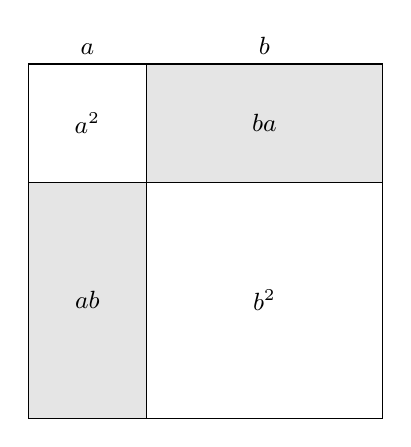
\begin{tikzpicture}[x=5mm, y=5mm,font=\small]
\definecolor{area}{gray}{0.9}
\draw(0,0) rectangle (9,9); 
\begin{scope}[fill=area, draw=black]
\filldraw (0,0) rectangle  (3,6);
\filldraw (3,6) rectangle (9,9);
\end{scope}

\node[above]  at (1.5,9) {$a$};
\node[above]  at (6,9) {$b$};
\node  at (1.5,7.5) {$a^2$};
\node  at (6,7.5) {$ba$};
\node  at (1.5,3) {$ab$};
\node  at (6,3) {$b^2$};	

\end{tikzpicture}}
\end{wrapfloat}

È possibile dare anche
un'interpretazione geometrica della 
formula~\(\tonda{A+B}^{2}=A^{2}+2{AB}+B^{2}\)
sostituendo~\(A\) e~\(B\) rispettivamente con le misure~\(a\) e~\(b\)
di due segmenti.

Prendiamo due segmenti di lunghezza~\(a\) e~\(b\), portiamo a
coincidere il secondo estremo del segmento lungo~\(a\) con il
primo estremo del segmento di lunghezza~\(b\): in questo modo
otteniamo un segmento di lunghezza~\(a+b\). Costruiamo il quadrato di
lato~\(a+b\), il quale avrà area~\((a+b)^{2}\) e dividiamolo come
nella figura a fianco.

Puoi notare che il quadrato di lato~\(a+b\) è composto da due quadrati
di area rispettivamente~\(a^{2}\) e~\(b^{2}\) e
da due rettangoli di area~\(ab\). Di conseguenza
l'area del quadrato è uguale 
a:~\((a+b)^{2}=a^{2}+b^{2}+{ab}+{ab}=a^{2}+2{ab}+b^{2}\).

\begin{esempio} Calcola il seguente quadrato:\\
\(\tonda{(3a^2-5ab}^2 = 9a^4 - 30 a^3 b + 25a^2 b^2\)
\end{esempio}

\begin{esempio} Trova quale quadrato dà come risultato il seguente 
trinomio:\\
\(9x^4 - 12 x^2 y + 4y^2= 
\tonda{3x^2}^2 +2\tonda{3x^2}\tonda{-2y}+\tonda{-2y}^2=
\tonda{3x^2-2y}^2\)
\end{esempio}

% \vspazio\ovalbox{\risolvii \ref{ese:11.1}, \ref{ese:11.2}, 
% \ref{ese:11.3}, \ref{ese:11.4}, \ref{ese:11.5}, \ref{ese:11.6}, 
% \ref{ese:11.7}, \ref{ese:11.8}, \ref{ese:11.9}, \ref{ese:11.10}}

\subsection{Quadrato di un polinomio}
\label{subsec:11_prodnot_quadratopolinomio}

Si consideri il trinomio~\(A+B+C\), il suo quadrato sarà dato da:
\begin{align*}
\tonda{A+B+C}^{2}&=\tonda{A+B+C}\cdot\tonda{A+B+C}\\
&=A^{2}+{AB}+{AC}+{BA}+B^{2}+{BC}+{CA}+{CB}+C^{2}\\
&=A^{2}+B^{2}+C^{2}+2{AB}+2{AC}+2{BC}.
\end{align*}


Peciò: \quad
\(\tonda{A+B+C}^{2}=A^{2}+B^{2}+C^{2}+2{AB}+2{AC}+2{BC}\)

\osservazione Il quadrato di un polinomio è uguale alla somma
dei quadrati dei monomi che lo compongono e dei doppi prodotti di ogni
termine per ciascuno dei successivi.

Nel caso di un polinomio composto da quattro monomi si ha:
\[\tonda{x+y+z+t}^{2}=x^{2}+y^{2}+z^{2}+t^{2}+2{xy}+2{xz}+2{xt}+2{yz}+2
{yt}+2{zt}.\]

\begin{esempio} Calcola il seguente quadrato:\\
\(\tonda{2a^3-4b-c}^2 = 4a^6 + 16b^2 +c^2 -16a^3 b -4 a^3 c +8 bc\)
\end{esempio}

\begin{esempio} Trova quale quadrato dà come risultato il seguente 
polinomio:\\
\(x^2 + 4y^2 + z^2 -4xy +2xz -4yz = \tonda{x-2y+z}^2\)
\end{esempio}

% \ovalbox{\risolvii \ref{ese:11.11}, \ref{ese:11.12}, \ref{ese:11.13}, 
% \ref{ese:11.14}, \ref{ese:11.15}}

\subsection{Prodotto della somma fra due monomi per la loro differenza}
\label{subsec:11_prodnot_sommaperdifferenza}

Osserviamo i seguenti prodotti:
\begin{align*}
\tonda{A-B}\tonda{A+B}   &= A^{2}+{AB}-{AB}-B^{2}=A^{2}-B^{2}\\
\tonda{-A+B}\tonda{A+B}  &= -A^{2}-{AB}+{AB}+B^{2}=-A^{2}+B^{2}\\
\tonda{-A+B}\tonda{-A-B} &= A^{2}+{AB}-{AB}-B^{2}=A^{2}-B^{2}\\
\tonda{A-B}\tonda{-A-B}  &= A^{2}-{AB}+{AB}-B^{2}=-A^{2}+B^{2}\\
\end{align*}

Quando eseguiamo il prodotto tra due binomi che hanno due
termini uguali e due termini opposti i prodotti incrociati si annullano
e rimangono i due prodotti del termine uguale per se stesso e dei due
termini opposti, il primo prodotto tra i due termini che non cambiano 
segno risulterà positivo, il prodotto tra i termini che cambiano segno 
risulterà negativo. 

\osservazione Il prodotto tra due binomi che hanno due termini
uguali e due termini opposti si ottiene moltiplicando tra di loro i due 
termini uguali e i due termini opposti.

% \begin{exrig}
\begin{esempio}
Alcuni esempi:
\begin{enumerate}
\item \(\tonda{3a^{2}+5{ab}} \tonda{3a^{2}-5{ab}}=9a^{2}-25a^{2}b^{2}\)
\item \(9a^2b^4-4x^6 = \tonda{3ab^{2}+2x^3} \tonda{3ab^{2}-2x^3}\)
\item \(\tonda{-{\dfrac{1}{4}}x^{2}+b}\cdot \tonda{+{\dfrac{1}{4}}x^{2}+b}=
        -\dfrac{1}{16}x^{4}+b^{2}\)
\item calcola il prodotto~\(28 \cdot 32\):~~
svolgimento:~\(28\cdot 32=(30-2)(30+2)=900-4=896\)
\item \((2x+1-y)(2x+1+y)=\)
\(\tonda{(\underbrace{2x+1}_{A})-\underbrace{y}_{B}}
  \tonda{(\underbrace{2x+1}_{A})+\underbrace{y}_{B}}= \newline
\hspace*{36.5mm}
=\underbrace{(2x+1)^{2}}_{A^{2}}-\underbrace{y^{2}}_{B^{2}}=
4x^{2}+4x+1-y^{2}\)
\end{enumerate}
\end{esempio}

% \end{exrig}

% \ovalbox{\risolvii \ref{ese:11.16}, \ref{ese:11.17}, \ref{ese:11.18}, 
% \ref{ese:11.19}, \ref{ese:11.20}, \ref{ese:11.21}, \ref{ese:11.22}, 
% \ref{ese:11.23}}

\subsection{Prodotto particolare}
\label{subsec:11_prodnot_particolare}

Consideriamo la moltiplicazione tra due binomi di primo grado che hanno i 
coefficienti dei termini di primo grado uguali a uno:
\[\tonda{x +3} \tonda{x+4} = x^2 +3x +4x +12 = x^2 +7x +12\]
Ora generalizziamo il calcolo mettendo al posto dei numeri dei parametri:
\[\tonda{x +a} \tonda{x+b} = x^2 +ax +bx +ab = x^2 +\tonda{a+b}x +ab\]
Chiamando:\\
\(a+b=s\) \quad somma dei termini di grado zero e\\
\(ab=p\) \quad prodotto degli stessi due termini,\\
possiamo dire che il prodotto tra i due binomi è un trinomio di secondo 
grado che ha per coefficienti rispettivamente: \(\quad 1, \quad s,\quad p\).
\[\tonda{x +a} \tonda{x+b} = x^2 +sx +p\]

% \begin{exrig}
\begin{esempio}
Alcuni esempi:
\begin{enumerate}
\item \(\tonda{x+7} \tonda{x+5}\) \quad \(s=7+5=12\) ~~ e ~~ 
\(p=7 \cdot 5=35\): \quad \(\tonda{x+7} \tonda{x+5}=x^2+12x+35\)
\item \(\tonda{x-3} \tonda{x+5}\) \quad \(s=-3+5=+2\) ~~ e ~~ 
\(p=-3 \cdot 5=-15\):\quad \(\tonda{x-3} \tonda{x+5}=x^2+2x-15\)
\item \(\tonda{x-4} \tonda{x-6}\) \quad \(s=-4-6=-10\) ~~ e ~~ 
\(p=-4 \cdot \tonda{-6}=+24\): \quad \(\tonda{x-4} \tonda{x-6}=x^2-10x+24\)
\item \(\tonda{x-3} \tonda{x+3}\) \quad \(s=-3+3=0\) ~~ e ~~ 
\(p=-3 \cdot 3=9\): \quad \(\tonda{x-3} \tonda{x+3}=x^2+9\)
\item \(\tonda{x-3} \tonda{x-3}\) \quad \(s=-3-3=-6\) ~~ e ~~ 
\(p=-3 \cdot 3=9\): \quad \(\tonda{x-3} \tonda{x-3}=x^2-6x+9\)
\end{enumerate}

\osservazione
I prodotti notevoli ``somma per differenza'' e ``quadrato del binomio'' 
possono essere visti come un caso particolare di trinomio particolare.
\end{esempio}

\begin{esempio}
Trova la moltiplicazione di binomi che dia il seguente trinomio:
\(x^2+3x-40\)\\
Devo trovare i due numeri \(a\) e \(b\) tali che: 
\(a+b=+3\) e \(a \cdot b=-40\). \\
Si inizia sempre dal valore assoluto del prodotto:\quad
\(40 = 1 \cdot 40; \quad 2 \cdot 20; \quad 4 \cdot 10; \quad 5 \cdot 8;~
\dots\)\\
I due fattori che hanno per somma algebrica \(3\) sono : \(5\) e \(8\).\\
Inseriamoli nello schema della moltiplicazione: \quad
\(\tonda{x \quad 5} \tonda{x \quad 8}\)\\
Ora aggiustiamo i segni in modo che 
la somma sia \(+3\) e il prodotto \(-40\):\\[-1em]
\begin{center}\(x^2+3x-40 = \tonda{x-5} \tonda{x+8}\)\end{center}
\end{esempio}
% \end{exrig}

\subsection{Cubo di un binomio}
\label{subsec:11_prodnot_cubo}

Si consideri il binomio~\(A+B\), il suo cubo sarà dato da:

\begin{align*}
\tonda{A+B}^{3}&=\tonda{A+B}^{2}\tonda{A+B}=\tonda{A^{2}+2{AB}
+B^{2}}\tonda{A+B}\\
%\tonda{A+B}^{3}&=\tonda{A+B}^{2}\tonda{A+B}\\
%&=\tonda{A^{2}+2{AB}+B^{2}}\tonda{A+B}\\
&=A^{3}+A^{2}B+2A^{2}B+2{AB}^{2}+{AB}^{2}+B^{3}\\
&=A^{3}+3A^{2}B+3{AB}^{2}+B^{3}.
\end{align*}

Pertanto, senza eseguire i passaggi intermedi si ha
\(\tonda{A+B}^{3}=A^{3}+3A^{2}B+3{AB}^{2}+B^{3}\).

\osservazione Il cubo di un binomio è uguale alla somma tra il
cubo del primo monomio, il triplo prodotto del quadrato del primo
monomio per il secondo, il triplo prodotto del quadrato del secondo
monomio per il primo e il cubo del secondo monomio.

Essendo~\(\tonda{A-B}^{3}=\left[A+\tonda{-B}\right]^{3}\), il
cubo della differenza di due monomi si ottiene facilmente dal cubo
della somma, quindi
\(\tonda{A-B}^{3}=A^{3}-3A^{2}B+3{AB}^{2}-B^{3}\).

\begin{esempio} Calcola i seguenti cubi di binomi:
\begin{multicols}{2}
\begin{enumeratea}
\item \(\tonda{x-2}^3= x^3-6x^2+12x-8\)
\item \(\tonda{-x+1}^3= -x^3+3x^2-3x+1\)
\item \(\tonda{-x-4}^3= -x^3-12x^2-48x-64\)
\item \(\tonda{2x+3y}^3= 8x^3+12x^2y+18xy^2+27\)
\end{enumeratea}
\end{multicols}
\end{esempio}

\begin{esempio}
Trova il cubo del binomio equivalente al seguente quadrinomio:\\
\(x^3-9x^2a+27xa^2-27a^3\)\\
Osserviamo che: \(x^3\) è il cubo di \(x\) \quad 
e \quad \(-27a^3\) è il cubo di \(-3a\)\\
possiamo sospettare che: \(x^3-9x^2a+27xa^2-27a^3 = \tonda{x-3a}^3\)\\
eseguendo il prodotto notevole, ne abbiamo la conferma.
\end{esempio}

% \vspazio\ovalbox{\risolvii \ref{ese:11.24}, \ref{ese:11.25}, 
% \ref{ese:11.26}, \ref{ese:11.27}}

\subsection{Potenza n-esima di un binomio}
\label{subsec:11_prodnot_potenzabinomio}

\affiancati{.59}{.39}{
Finora abbiamo calcolato le potenze del binomio~\(a+b\) fino
all'ordine tre, in questo paragrafo ci si propone di
fornire un criterio che permetta di calcolare la potenza~\((a+b)^{n}\),
con~\(n\in \insN\). Osserviamo le potenze ottenute:
}{
\begin{multline*}
\\(a+b)^{0}=1\\
(a+b)^{1}=a+b\\
(a+b)^{2}=a^{2}+2{ab}+b^{2}\\
(a+b)^{3}=a^{3}+3a^{2}b+3{ab}^{2}+b^{3}.\\
\end{multline*}
}
Si può notare che:

\begin{itemize*}
\item lo sviluppo di ciascuna potenza dà origine a un polinomio
omogeneo dello stesso grado dell'esponente della
potenza, completo e ordinato secondo le potenze decrescenti di~\(a\) e 
crescenti di~\(b\)
\item il primo coefficiente è sempre uguale a~1;
\item i coefficienti di ciascuna riga si ottengono utilizzando una
disposizione dei numeri a triangolo, detto \emph{triangolo di Tartaglia}.
\end{itemize*}

\begin{inaccessibleblock}[Il triangolo di Tartaglia]
\begin{minipage}[t]{.49\textwidth}
 \centering  \begin{tikzpicture}[x=9mm,y=5mm]

  \tikzset{box/.style={
      minimum height=5mm,
      inner sep=.7mm,
      outer sep=0mm,
      text width=10mm,
      text centered,
      font=\small\ttfamily,
      line width=.25mm,
   }
} 
 \node[box=odd] (p-0-0) at (0,0) {1};
  \foreach \linea in {1,...,6} {
    \node[box=odd] (p-\linea-0) at (-\linea/2,-\linea) {1};
    \pgfmathsetmacro{\valore}{1};
    \foreach \col in {1,...,\linea} {
      \pgfmathtruncatemacro{\valore}{\valore*((\linea-\col+1)/\col)+0.5};
      \global\let\valore=\valore
      \coordinate (pos) at (-\linea/2+\col,-\linea);
      \pgfmathtruncatemacro{\rest}{mod(\valore,2)}
      \ifnum \rest=0
        \node[box=even] (p-\linea-\col) at (pos) {\valore};
      \else
        \node[box=odd] (p-\linea-\col) at (pos) {\valore};
      \fi
    }
  }
\end{tikzpicture}
\end{minipage}
\hfil
 \begin{minipage}[t]{.49\textwidth}
 \centering \begin{tikzpicture}[x=12mm,y=8mm]
  \tikzset{
    box/.style={
      minimum height=5mm,
      inner sep=.7mm,
      outer sep=0mm,
      text width=10mm,
      text centered,
      font=\small\ttfamily,
      line width=.25mm,
    },
    link/.style={->,blue,line width=.3mm},
    plus/.style={text=red,font=\small\ttfamily}
  }
 
  \node[box=odd] (p-0-0) at (0,0) {1};
  \foreach \linea in {1,...,4} {
    \node[box=odd] (p-\linea-0) at (-\linea/2,-\linea) {1};
    \pgfmathsetmacro{\valore}{1};
    \foreach \col in {1,...,\linea} {
      \pgfmathtruncatemacro{\valore}{\valore*((\linea-\col+1)/\col)+0.5};
      \global\let\valore=\valore
      \coordinate (pos) at (-\linea/2+\col,-\linea);
      \pgfmathtruncatemacro{\rest}{mod(\valore,2)}
      \ifnum \rest=0
        \node[box=even] (p-\linea-\col) at (pos) {\valore};
      \else
        \node[box=odd] (p-\linea-\col) at (pos) {\valore};
      \fi
      \ifnum \col<\linea
        \node[plus,above=0mm of p-\linea-\col]{+};
        \pgfmathtruncatemacro{\plinea}{\linea-1}
        \pgfmathtruncatemacro{\pcol}{\col-1}
        \draw[link] (p-\plinea-\pcol) -- (p-\linea-\col);
        \draw[link] ( p-\plinea-\col) -- (p-\linea-\col);
      \fi
    }
  }
\end{tikzpicture}
\end{minipage}
\end{inaccessibleblock}

In questo triangolo i numeri di ciascuna riga (tranne il primo e
l'ultimo che sono uguali a~1) sono la somma dei due
soprastanti della riga precedente.

Con questa semplice regola si hanno gli sviluppi:

\begin{itemize*}
\item \((a+b)^{0}=1\)
\item \((a+b)^{1}=a+b\)
\item \((a+b)^{2}=a^{2}+2{ab}+b^{2}\)
\item \((a+b)^{3}=a^{3}+3a^{2}b+3{ab}^{2}+b^{3}\)
\item \((a+b)^{4}=a^{4}+4a^{3}b+6a^{2}b^{2}+4{ab}^{3}+b^{4}\)
\item \((a+b)^{5}=a^{5}+5a^{4}b+10a^{3}b^{2}+10a^{2}b^{3}+5{ab}^{4}+b^{5}\).
\end{itemize*}

\begin{esempio} Calcola le seguenti potenze di binomi:
\begin{enumeratea}
\item \(\tonda{-3x-4}^0  = 1\)
\item \(\tonda{-5x+4}^1  = -5x+4\)
\item \(\tonda{-2x-3y}^2 = 4x^2+12xy+9y^2\)
\item \(\tonda{-2x-3y}^3 = -8x^3-36x^2y-54xy^2-27y^3\)
\item \(\tonda{x-2}^4    = x^4 -8x^3+24x^2-32x+16\)
\item \(\tonda{-x+1}^5   = -x^5 +5x^4-10x^3+10x^2-5x+1\)
\end{enumeratea}
\end{esempio}

% \ovalbox{\risolvii \ref{ese:11.28}, \ref{ese:11.29}, \ref{ese:11.30}}


